\section{Auswertung}
\subsection{Molwärme bei konstantem Druck}
Mit Hilfe der Formel
\begin{equation}
  C_p = \frac{E \cdot M}{\Delta T \cdot m}
\end{equation}
lässt sich die Molwärme unter konstantem Druck berechnen.
Es ist $E$ die zugeführte Energie, $M$ die molare Masse, $\Delta T$ die Temperaturänderung und $m$ die Masse der Probe.
Da die Größen $E$ und $\Delta{T}$ Messgrößen sind, die Messunsicherheiten besitzen,
lässt sich der Fehler für die Molwärme bei konstantem Druck mit Hilfe der Gaußschen Fehlerfortpflanzung durch
\begin{equation}
  \Gamma_{C_p} = \sqrt{ (\frac{M}{\Delta{T}\cdot{m}})^2\cdot(\Gamma_E)^2 + (\frac{E\cdot{M}}{(\Delta{T})^2\cdot{m}})^2\cdot(\Gamma_{\Delta{T}})^2 }
\end{equation}
berechnen.

Bei dem zu untersuchenden Material handelt es sich um Kupfer.
Die entsprechenden Werte für die molare Masse $M$ \cite{cu} und die Masse $m$ der Kupferprobe \cite{skript} sind
\begin{gather*}
  M_{\text{Cu}} = 63,546\frac{\text{g}}{\text{mol}} \\
  m_{\text{Cu}} = 342\si{\gram}.
\end{gather*}
Die Energie lässt sich durch
\begin{equation}
  E = U\cdot I\cdot \Delta t
\end{equation}
berechnen, wobei $U$ die aufgenommene Spannung, $I$ der gemessene Strom und $\Delta t$ das Intervall ist.
Da $U$, $I$ und $\Delta{t}$ Messunsicherheiten beinhalten,
lässt sich mittels Gaußscher Fehlerfortpflanzung der Fehler von $E$ mit der Formel
\begin{equation}
  \Gamma_E = \sqrt{ (I\cdot\Delta{t})^2\cdot(\Gamma_U)^2 + (U\cdot\Delta{t})^2\cdot(\Gamma_I)^2 + (U\cdot{I})^2\cdot(\Gamma_{\Delta{t}})^2 }
\end{equation}
berechnen.

Aus der Formel
\begin{equation}
  T = 0,00134R^2 + 2,296R - 243,02\text{°C}
\end{equation}
folgt nach der pq-Formel für die Widerstände die Formel
\begin{equation}
  R_+ = -\frac{2,296}{2\cdot0,00134} + \sqrt{ \left(\frac{2,296}{2\cdot0,00134}\right)^2 + \frac{243,02 + T}{0,00134} },
  \end{equation}
mit der sich die Widerstände des Thermoelements zur entsprechenden Temperatur berechnen lassen.
Der Tabelle \ref{tab:1} können die gemessenen Widerstände, Temperaturänderungen, Zeiten, Ströme, Spannungen, Energien und Molwärmen entnommen werden.

\begin{table}
[H]
\begin{tabular}{ccccccc}

  \toprule
$R$ [$\si{\ohm}$] & $\Delta{T}\pm\Gamma_{\Delta{T}}$ [°] & $t \pm \Gamma_t$ [s] & $I \pm \Gamma_I$ [mA] & $U \pm \Gamma_U$ [V] & $E \pm \Gamma_E$ [J] & $C_p \pm \Gamma_{C_p} $ [J/mol K]\\

\midrule
$21,1$ & $-            $ & $ -       $ & $0            $ & $0             $ & $-$            & $-$              \\

\textcolor{red}{$25,7$} & \textcolor{red}{$10,82 \pm 0,1$} & \textcolor{red}{$523 \pm 5$} & \textcolor{red}{$133,8 \pm 0,1$}
& \textcolor{red}{$13,80 \pm 0,01$} & \textcolor{red}{$ 966 \pm  9$}  & \textcolor{red}{$16,59 \pm 0,22$} \\

\textcolor{red}{$29,9$} & \textcolor{red}{$10,00 \pm 0,1$} & \textcolor{red}{$572 \pm 5$} & \textcolor{red}{$143,7 \pm 0,1$}
& \textcolor{red}{$13,88 \pm 0,01$} & \textcolor{red}{$1141 \pm 10$}  & \textcolor{red}{$21,20 \pm 0,28$} \\
\textcolor{red}{$34,1$} & \textcolor{red}{$10,00 \pm 0,1$} & \textcolor{red}{$610 \pm 5$} & \textcolor{red}{$145,8 \pm 0,1$}
& \textcolor{red}{$13,88 \pm 0,01$} & \textcolor{red}{$1234 \pm 10$}  & \textcolor{red}{$22,93 \pm 0,30$} \\
$38,3$ & $10,00 \pm 0,1$ & $577 \pm 5$ & $153,7 \pm 0,1$ & $16,20 \pm 0,01$ & $1437 \pm 13$  & $26,70 \pm 0,40$ \\

$42,4$ & $10,00 \pm 0,1$ & $378 \pm 5$ & $178,0 \pm 0,1$ & $18,75 \pm 0,01$ & $1262 \pm 17$  & $23,40 \pm 0,40$ \\

$46,6$ & $10,00 \pm 0,1$ & $365 \pm 5$ & $178,0 \pm 0,1$ & $18,75 \pm 0,01$ & $1218 \pm 17$  & $22,60 \pm 0,40$ \\

$50,7$ & $10,00 \pm 0,1$ & $327 \pm 5$ & $180,3 \pm 0,1$ & $19,03 \pm 0,01$ & $1122 \pm 17$  & $20,80 \pm 0,40$ \\

$54,8$ & $10,00 \pm 0,1$ & $315 \pm 5$ & $180,5 \pm 0,1$ & $19,60 \pm 0,01$ & $1114 \pm 18$  & $20,70 \pm 0,40$ \\

$58,9$ & $10,00 \pm 0,1$ & $375 \pm 5$ & $180,7 \pm 0,1$ & $19,08 \pm 0,01$ & $1293 \pm 17$  & $24,00 \pm 0,40$ \\

$63,0$ & $10,00 \pm 0,1$ & $376 \pm 5$ & $180,8 \pm 0,1$ & $19,10 \pm 0,01$ & $1298 \pm 17$  & $24,10 \pm 0,40$ \\

$67,0$ & $10,00 \pm 0,1$ & $384 \pm 5$ & $180,9 \pm 0,1$ & $19,12 \pm 0,01$ & $1328 \pm 17$  & $24,70 \pm 0,40$ \\

$71,0$ & $10,00 \pm 0,1$ & $406 \pm 5$ & $181,0 \pm 0,1$ & $19,13 \pm 0,01$ & $1406 \pm 17$  & $26,10 \pm 0,40$ \\

$75,1$ & $10,00 \pm 0,1$ & $397 \pm 5$ & $181,1 \pm 0,1$ & $19,10 \pm 0,01$ & $1373 \pm 17$  & $25,50 \pm 0,40$ \\

$79,0$ & $10,00 \pm 0,1$ & $361 \pm 5$ & $181,2 \pm 0,1$ & $19,14 \pm 0,01$ & $1252 \pm 17$  & $23,30 \pm 0,40$ \\

$83,0$ & $10,00 \pm 0,1$ & $346 \pm 5$ & $181,2 \pm 0,1$ & $19,14 \pm 0,01$ & $1200 \pm 17$  & $22,30 \pm 0,40$ \\

$87,0$ & $10,00 \pm 0,1$ & $299 \pm 5$ & $181,2 \pm 0,1$ & $19,14 \pm 0,01$ & $1037 \pm 17$  & $19,30 \pm 0,40$ \\

$90,9$ & $10,00 \pm 0,1$ & $275 \pm 5$ & $181,3 \pm 0,1$ & $19,15 \pm 0,01$ & $ 955 \pm 17$  & $17,70 \pm 0,40$ \\

$94,9$ & $10,00 \pm 0,1$ & $328 \pm 5$ & $181,3 \pm 0,1$ & $19,14 \pm 0,01$ & $1138 \pm 17$  & $21,10 \pm 0,40$ \\

$98,8$ & $10,00 \pm 0,1$ & $383 \pm 5$ & $181,4 \pm 0,1$ & $19,14 \pm 0,01$ & $1330 \pm 17$  & $24,70 \pm 0,40$ \\

$102,7$ & $10,00 \pm 0,1$ & $411 \pm 5$ & $181,4 \pm 0,1$ & $19,13 \pm 0,01$ & $1426 \pm 17$ & $26,50 \pm 0,40$ \\

$106,6$ & $10,00 \pm 0,1$ & $358 \pm 5$ & $181,4 \pm 0,1$ & $19,13 \pm 0,01$ & $1242 \pm 17$ & $23,10 \pm 0,40$ \\

$110,4$ & $10,00 \pm 0,1$ & $361 \pm 5$ & $181,5 \pm 0,1$ & $19,12 \pm 0,01$ & $1253 \pm 17$ & $23,30 \pm 0,40$ \\

\bottomrule
\end{tabular}

\caption{Überblick über die gemessenen und berechneten Daten.}
\label{tab:1}
\end{table}



\subsection{Molwärme bei konstantem Volumen}
Mit Hilfe der Formel
\begin{equation}
  C_V = C_p - 9\alpha^2\kappa{V_0}T
\end{equation}
lässt sich die Molwärme bei konstantem Volumen berechnen.
Dabei ist $\alpha$ der lineare Ausdehnungskoeffizient, $\kappa = 140$GPa der Kompressionsmodul \cite{kappa}, $V_0 = 7,10\frac{\text{cm}^3}{\text{mol}}$ das Molvolumen \cite{cu} und T die Temperatur.
Der Fehler ist
\begin{equation}
  \Gamma_{C_V} = \Gamma_{C_p}.
\end{equation}
Der lineare Ausdehnungskoeffizient lässt sich der Tabelle in Abbildung \ref{alpha} entnehmen.

\begin{figure}[H]
  \centering
  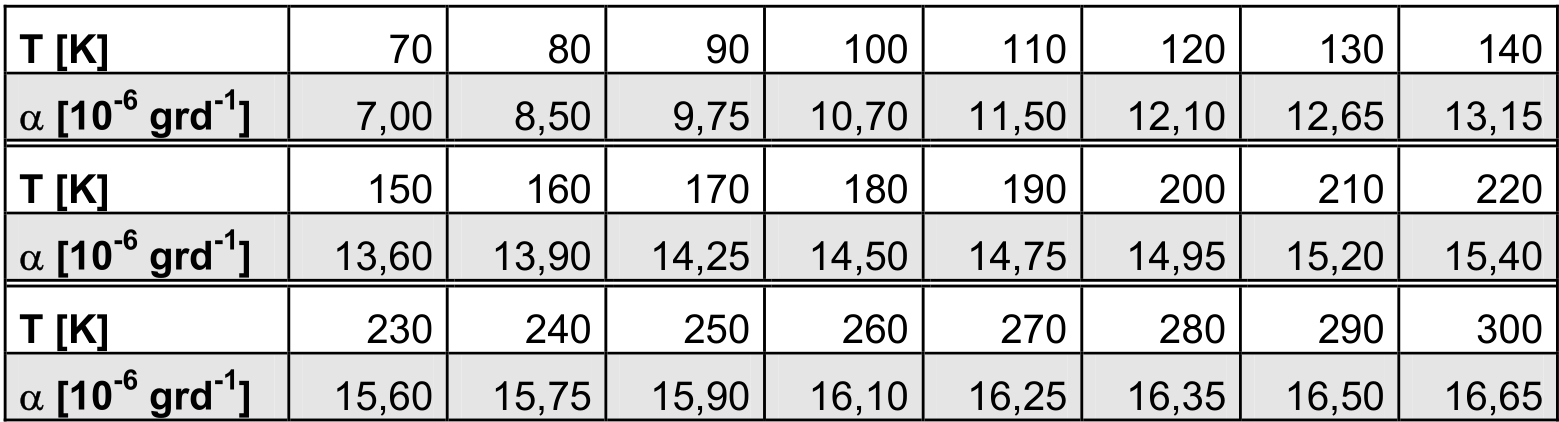
\includegraphics[width=\textwidth]{alpha.png}
  \caption{Linearer Ausdehnungskoeffizient $\alpha$ von Kupfer in Abhängigkeit von der Temperatur. \cite{skript}}
  \label{alpha}
\end{figure}

Zur Berechnung der theoretischen Molwärme wird Formel \eqref{eqn:debye} verwendet.
Dabei beträgt die Debye-Temperatur $\theta_D = 345$K \cite{debye}.
Die allgemeine Gaskonstante beträgt $R = 8,31\frac{\text{J}}{\text{mol}\cdot\text{K}}$ \cite[587]{dem}.
In der folgenden Tabelle \ref{tab:2} können die empirischen und theoretischen Molwärmen entnommen werden.

\begin{table}[H]
  \centering
  \begin{tabular}{ccccc}
    \toprule
    $T$ [K] & $C_p \pm \Gamma_{C_p} $ [J/mol K]
    & $C_V \pm \Gamma_{C_V} $ [J/mol K] & $C_{V}^{\text{Theorie}}$ [J/mol K] \\
    \midrule
    $ 90$ & $16,59 \pm 0,22$ & $16,51 \pm 0,22$ & 13,18 \\
    $100$ & $21,20 \pm 0,28$ & $21,10 \pm 0,28$ & 14,68 \\
    $110$ & $22,93 \pm 0,30$ & $22,80 \pm 0,30$ & 15,96 \\
    $120$ & $26,70 \pm 0,40$ & $26,54 \pm 0,40$ & 17,05 \\
    $130$ & $23,40 \pm 0,40$ & $23,21 \pm 0,40$ & 17,97 \\
    $140$ & $22,60 \pm 0,40$ & $22,38 \pm 0,40$ & 18,67 \\
    $150$ & $20,80 \pm 0,40$ & $20,55 \pm 0,40$ & 19,42 \\
    $160$ & $20,70 \pm 0,40$ & $20,42 \pm 0,40$ & 19,98 \\
    $170$ & $24,00 \pm 0,40$ & $23,69 \pm 0,40$ & 20,46 \\
    $180$ & $24,10 \pm 0,40$ & $23,76 \pm 0,40$ & 20,92 \\
    $190$ & $24,70 \pm 0,40$ & $24,33 \pm 0,40$ & 21,27 \\
    $200$ & $26,10 \pm 0,40$ & $25,70 \pm 0,40$ & 21,59 \\
    $210$ & $25,50 \pm 0,40$ & $25,07 \pm 0,40$ & 21,89 \\
    $220$ & $23,30 \pm 0,40$ & $22,83 \pm 0,40$ & 22,12 \\
    $230$ & $22,30 \pm 0,40$ & $21,80 \pm 0,40$ & 22,35 \\
    $240$ & $19,30 \pm 0,40$ & $18,77 \pm 0,40$ & 22,65 \\
    $250$ & $17,70 \pm 0,40$ & $17,13 \pm 0,40$ & 22,71 \\
    $260$ & $21,10 \pm 0,40$ & $20,50 \pm 0,40$ & 23,03 \\
    $270$ & $24,70 \pm 0,40$ & $24,06 \pm 0,40$ & 23,14 \\
    $280$ & $26,50 \pm 0,40$ & $25,83 \pm 0,40$ & 23,04 \\
    $290$ & $23,10 \pm 0,40$ & $22,39 \pm 0,40$ & 23,29 \\
    $300$ & $23,30 \pm 0,40$ & $22,56 \pm 0,40$ & 23,37 \\
    \bottomrule
  \end{tabular}
  \caption{Empirische und theoretische Molwärmen im Vergleich}
  \label{tab:2}
\end{table}

In Abbildung \ref{C_V} werden die berechneten Werte der Molwärme bei konstantem Volumen gegen die Temperatur aufgetragen.

\begin{figure}[H]
  \centering
  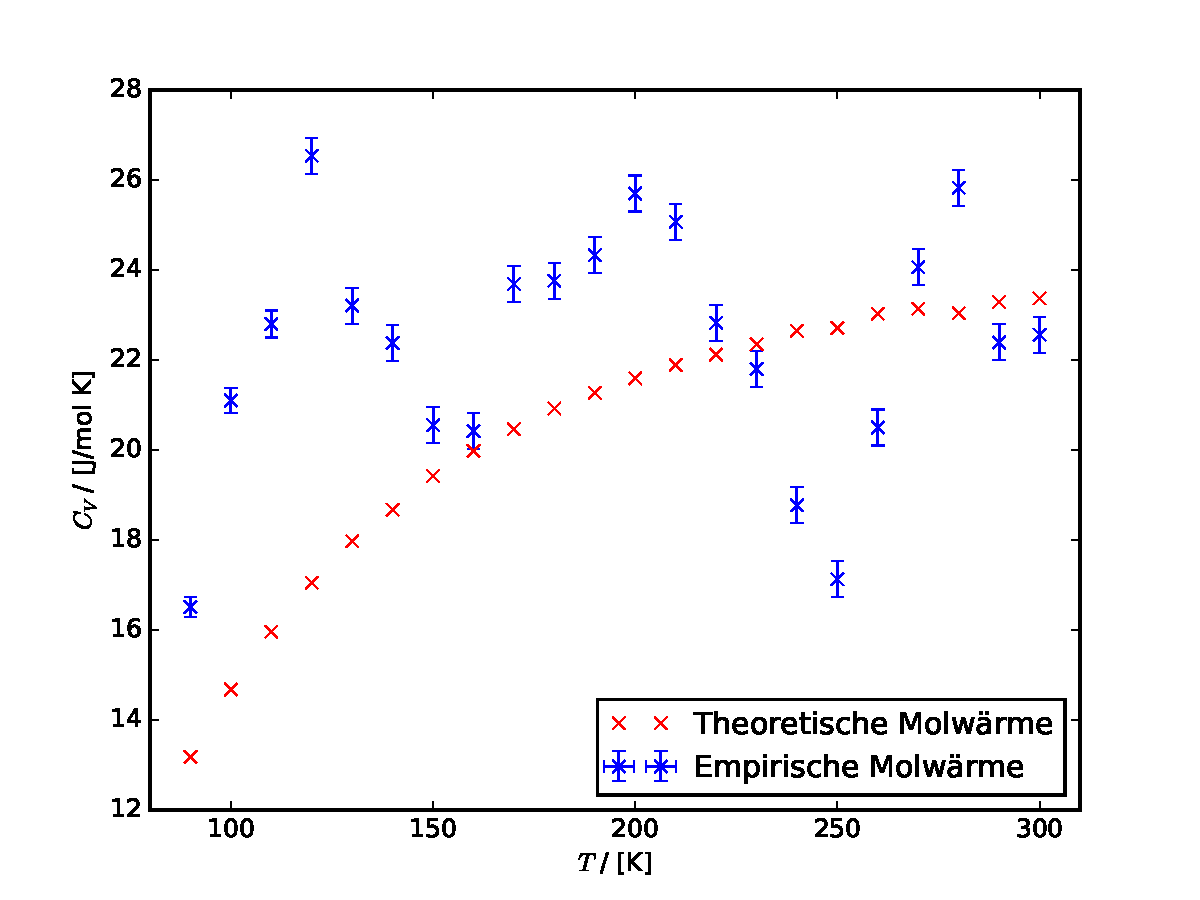
\includegraphics[width=\textwidth]{C_V_T.pdf}
  \caption{Empirische und theoretisch berechnete Molwärmen im Vergleich.}
  \label{C_V}
\end{figure}

\subsection{Debye-Temperatur}
\subsubsection{Empirisch}

Der Tabelle in Abbildung \ref{debfkt} können die Zahlenwerte der universellen Debye-Kurve durch lineare Interpolation entnommen werden.

\begin{figure}[H]
  \centering
  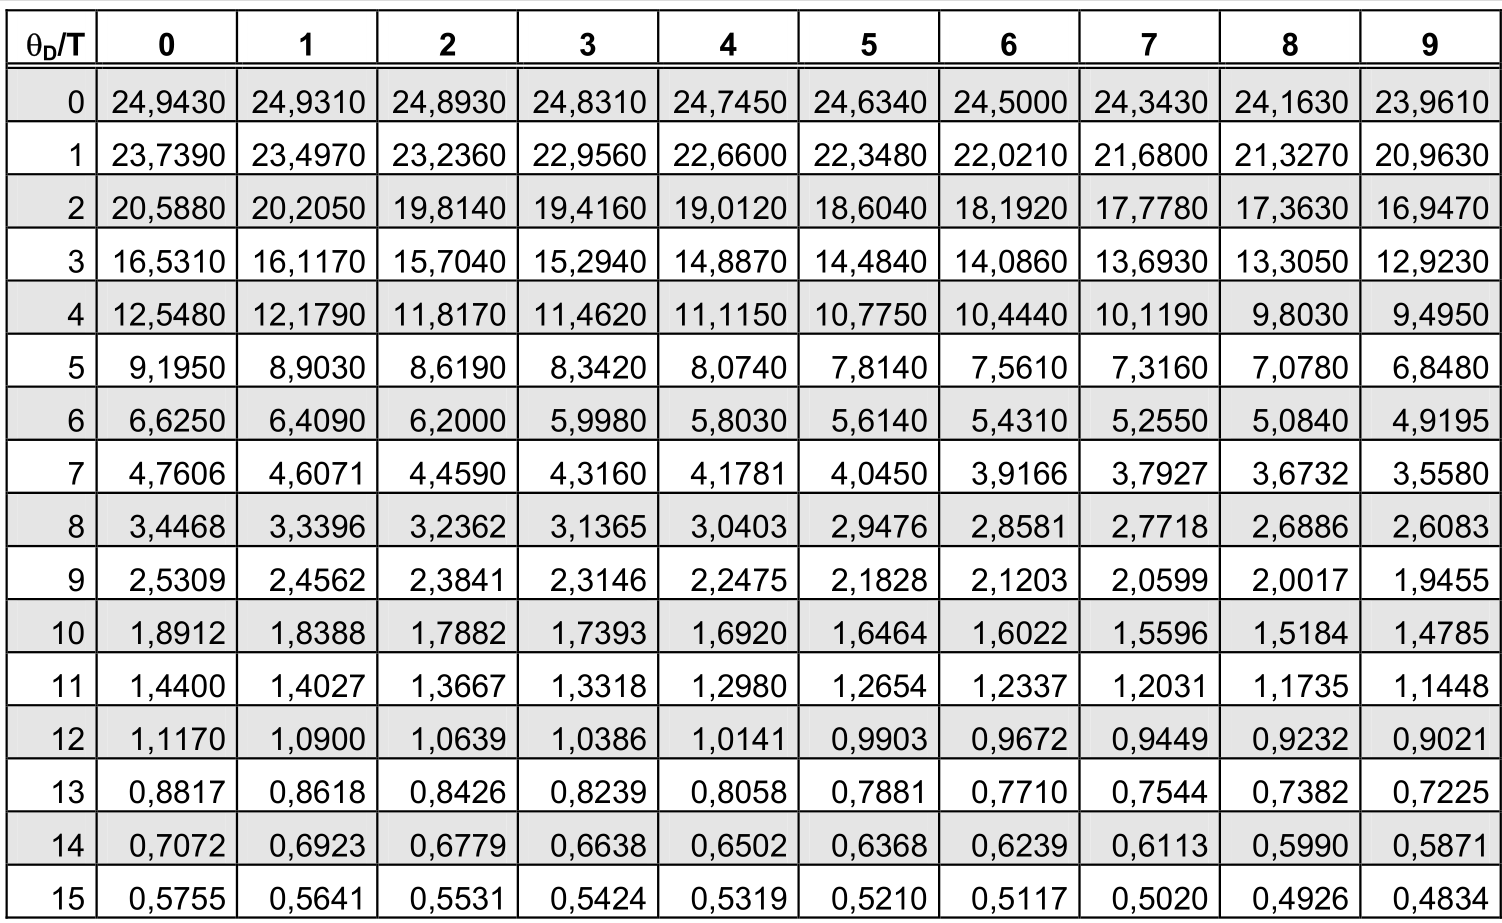
\includegraphics[width=12cm]{debtab.png}
  \caption{Zahlenwerte der Debye-Funktion für $R = 8,31439\frac{\text{J}}{\text{mol}\cdot\text{K}}$. Molwärme $C_V$ in $\frac{\text{J}}{\text{mol}\cdot\text{K}}$. \cite{skript}}
  \label{debfkt}
\end{figure}

Zu den gemessenen ($C_V,T$)-Wertepaaren werden die Werte der Debye-Kurve mit den entsprechenden Temperaturen multipliziert.
Es werden nur die Messwerte bis $T_{\text{max}} = 170$K berücksichtigt.
In Tabelle \ref{tab:3} können die Debye-Temperaturen zu den gemessenen $(C_V,T)$-Wertepaaren mit Hilfe der Debye-Kurve entnommen werden.

\begin{table}[H]
  \centering
  \begin{tabular}{cccc}
    \toprule
    $C_V$ [$\frac{\text{J}}{\text{mol}\cdot\text{K}}$] & T [K] & $\frac{\theta_D}{T}$ & $\theta_D$ [K] \\
    \midrule
    $16,51 \pm 0,22$ & $ 90$ & 3,01 & 270,47 \\
    $21,10 \pm 0,28$ & $100$ & 1,84 & 183,75 \\
    $22,80 \pm 0,30$ & $110$ & 1,30 & 142,78 \\
    $26,54 \pm 0,40$ & $120$ & 1,33 & 159,17 \\
    $23,21 \pm 0,40$ & $130$ & 1,17 & 151,82 \\
    $22,38 \pm 0,40$ & $140$ & 1,43 & 200,38 \\
    $20,55 \pm 0,40$ & $150$ & 2,01 & 301,35 \\
    $20,42 \pm 0,40$ & $160$ & 2,04 & 326,63 \\
    $23,69 \pm 0,40$ & $170$ & 1,02 & 172,64 \\
    \bottomrule
  \end{tabular}
  \caption{Bestimmte Debye-Temperaturen zu den gemessenen $(C_V,T)$-Wertepaaren mit Hilfe der Debye-Kurve.}
  \label{tab:3}
\end{table}

Gemittelt ergibt sich eine Debye-Temperatur mit einer Standardabweichung von
\begin{align*}
  \overline{\theta_D} \pm \Gamma_{\overline{\theta_D}} = (212,11 \pm 23,04)\text{K}.
  \end{align*}

\subsubsection{Theoretisch}
Aus der Formel \eqref{eqn:omega} lässt sich die Debye-Frequenz $\omega_D$ berechnen.
Für die Geschwindigkeiten der Longitudinal- bzw Transversalwellen gilt \cite{skript}
\begin{align*}
  v_{\text{long}} = 4700\text{m{/s}}, \\
  v_{\text{trans}} = 2260\text{m/s}.
\end{align*}
Außerdem gilt
\begin{gather*}
  L = \left({\frac{m}{\rho}}\right)^{\frac{1}{3}} = 0,0337\text{m}, \\
  N_L = \frac{N_A \cdot m}{V_0 \cdot \rho} = \frac{3,2374\cdot10^{24}}{\text{m}^3},
\end{gather*}
wobei $\rho = 8,96 \text{g}/\text{cm}^3$ die Dichte von Kupfer \cite{cu}, $m = 342$g die Masse der Kupferprobe \cite{skript},
$N_A = \frac{6,022\cdot10^{23}}{\text{mol}}$ die Avogadro-Konstante \cite{dem} und $V_0$ das Molvolumen ist (s.o.).
Damit ergibt sich die Debye-Frequenz von
\begin{align*}
  \omega_D^{\text{Theorie}} = 5,3844\cdot10^{13}\text{Hz}.
\end{align*}
Aus der Relation
\begin{equation}
  \theta_D = \frac{\hbar\omega_D}{k_B}
\end{equation}
folgt für die Debye-Temperatur
\begin{align*}
  \theta_D^{\text{Theorie}} = 411,27\text{K}.
\end{align*}
